
\section{Further Work}
This section details some areas which given additional time to work on the project would at the very least be investigated, if not implemented. Each of these areas would hopefully provide some benefit in assisting to demonstrate the possibilities of hybrid methods.

\subsection{Gathering feedback from experienced engineers}
Approaching the end of the project it became clear that in order to better identify the systems strengths and weaknesses would require additional user testing by engineers who have experience conducting this type of analysis. Despite a lack of available time obtaining feedback from engineers with extensive applied industrial experience along with that of academics would have hopefully allowed for a more conclusive analysis of the systems and its ability to work across a greater number of general case scenarios. 

Part of the reason feedback for not obtaining user feedback was the difficulty of doing so given the available time available simply to implement the project and validate it for a selection of basic models. As such even if time had been available the ethical clearance required to collect user feedback at the start was not obtained.


\subsection{Improving usability through a web interface}
Although possible to visit various engineers in order to conduct feedback the process is both time consuming on my part and inconvenient for the participant as a rigid time for which to meet must be scheduled and a laptop containing the working software brought to them which they must design or transfer their model to before running it multiple times to obtain results. This scenario is at best inconvenient for the participants and pressures them into arriving at a conclusion within a relatively small time of experimenting with it. \\ 

\noindent
Instead by facilitating interaction with the system by means of a web interface the engineers would be able spend as little or as much time as they like experimenting with the system and allow them to submit feedback digitally allowing feedback to be obtained and aggregated from a much wider range of different sources separated by significant geographic distance. \\\ 

\noindent
To use the interface an engineer would simply need to submit a model they have already created  along with a JSON file containing edges they have designated as important for their model. LISA supports imports from multiple CAD formats including Standard for the Exchange of Product model data (STEP) and Initial Graphics Exchange Specification (IGES)) \cite{LISAManual}. Upon receiving the request the web server would the current project with their input data and having finished allow them to download the re meshed model along with the calculated stress data for analysis.


\section{Personal Reflections and Summary}
%Comparing the current progress of the project against the plan things are on track to be completed as scheduled. So far I am pleased with both my research efforts and the functionality that I have been able to implement. My primary concern at present is that the ILP generated rules may not perform as well as expected when fully implemented or that they perform well but only for a limited set of geometries, which would be disappointing. While conducting research, development and implementation for the project I have worked methodically to best understand each problem as and when they occur and consider each of the possible solutions before committing to one. I feel this approached has saved me much time and has forced me to reach a better view about what exactly each subsystem should do and how to implement it. In hindsight if I were to repeat the first part of the project again I would have organised my time differently to spend less of it focussed on the details of coursework assignments for other modules into making further progress on the implementation of the rule system.

\noindent
Overall I felt the project was a success. The final software solution was evidently capable of facilitating execution and therefore allowing comparison to be made of both heuristic and stress based mesh refinement techniques. Not only did the final system allow this comparison for the two specific approaches that were coded by me in order to validate the system it provided a flexible framework allowing for a potentially unlimited set of configurations when performing future experimentation. \\ 

\noindent
From my perspective I wanted to use this project as an opportunity to improve my understanding of a technology that I previously had limited knowledge of through its use on my industrial placement year. My prior experience with with FE analysis was very much confined to that of a typical engineer making use of the method through a licensed desktop application with many of the technicalities that are of most interest to a computer scientist hidden. I therefore found the project highly enjoyable as an opportunity to learn more about the underlying processes through both research and practical experimentation. As a means of facilitating my own learning as an individual I therefore also consider the project a success.

\noindent
Despite working on larger software projects during my year within industry this was certainly the most complex I have undertaken as an individual. As the lead software developer on my own project I encountered many challenges which as a junior developer within industry were not my responsibility but which I observed team leaders and senior developers encountering regularly. Such tasks were those that required high level analysis of the overall solution in order to continuously steer the project in the right direction and ensure successful delivery within the specified time scales. In many ways the project therefore gave me a good appreciation of the overall difficulties associated with delivering a software project in its entirety and one that has the potential change fluidly throughout.\\ 

\noindent
In particular I found the research and evaluation phases particularly difficult. Upon completion I came to realise this was largely due to my lack of formal education in mechanical engineering which meant I had to work a lot harder both to understand the initial problems associated with the methods and subsequently to correctly evaluate the results I obtained. Had I chosen a more traditional computer science topic I believe both of these aspects would have been much easier.

Having completed the research too much time was then spent concerned with specifics of the implementation. 




A negative consequence of the bespoke nature of the system was that obtaining details of designs results for comparable systems published by the wider academic community was both challenging and highly time consuming.  \\ 

\noindent
Throughout the majority of the project I felt organisation of time and planning of activities was done well. Work on the project began early with the goal of easing pressure in the later stages and work continued despite deadlines for coursework associated with other modules. A crucial mistake made was to reduce effort two months before the deadline having completed the software implementation and written much of the initial sections of the dissertation despite not completing evaluation of the results. Evaluation of the software turned out to be substantially more time consuming than expected in additional stresses towards the deadline. \\

\noindent
Given the chance to redo the project I would have liked to conducted more research to better assess an even wider scope of research surrounding meshing methods. In many cases the academic literature surrounding bespoke meshing techniques became complicated very quickly and was clearly aimed at individuals with a high degree of prior experience.

%A consequence of this was I  opted for the simplest version of the two approaches I could find so as to tesy my


By contrast I found the system design and programming components 


planning and research components 

managerial architectural aspects which I had not previously had that great an involvement with
%Mention difficulty in initially predicting the unforseen technical challenges.

%Describe ambition behind project to challenge both comptuer science skills and improve knowledge of software methods for solving mechanical engineering problems.

%To understand various mechanical engineering problems for which finite element analysis is used and use this knowledge to guide my decisions as a software engineer when implementing the various methods was challenging and often time consuming given that I did not have a particularly deep background of the topics, made correct evaluation of the software towards the end of the project challenging.


%Things that went well
% - Generally organised time well, made a good start at the beginning of the year when there was little coursework to do.

%spent about a month and a half just readings without trying to implement anything - despite there being not that many papers on topics specific to this worked hard to find a wide variery of approaches taken by people and develop a clear understanding of the topic.


% - Tried to approach the development of the system as a piece of industrial software, tried to adopt SOLID principals wherever possible which resulted in a system that was actually well structured and highly extendable.


%Things I would do better
%Spend less time working on the initial structuere and design, gone for minimum viable product in the eairly stages of development and then spent more time in the evaluation/ refinement stages in order to try and better understand how to improve the methods for particular scenarios.

% I actually spent much longer doing the groundwork required to implement the cool stuff than I had previously expected, designing the data model and writing the various code required for general meshing proved more problematic than originally anticipated.

% Although very keen to utilise functional programming features as much as possible at the start I realised towards the end of the project that doing this a lot can actually make you as a programmer very lazy and in some cases can make code more challenging to read for those who aren't familiar with the style. Having completed this project I now feel I have a better appreciation of where to use functional programming best and when to best avoid it in order to improve speed and readability.

\newpage
\pagestyle{empty}
\begin{landscape}
\vspace*{1cm}
\hspace*{-3cm}
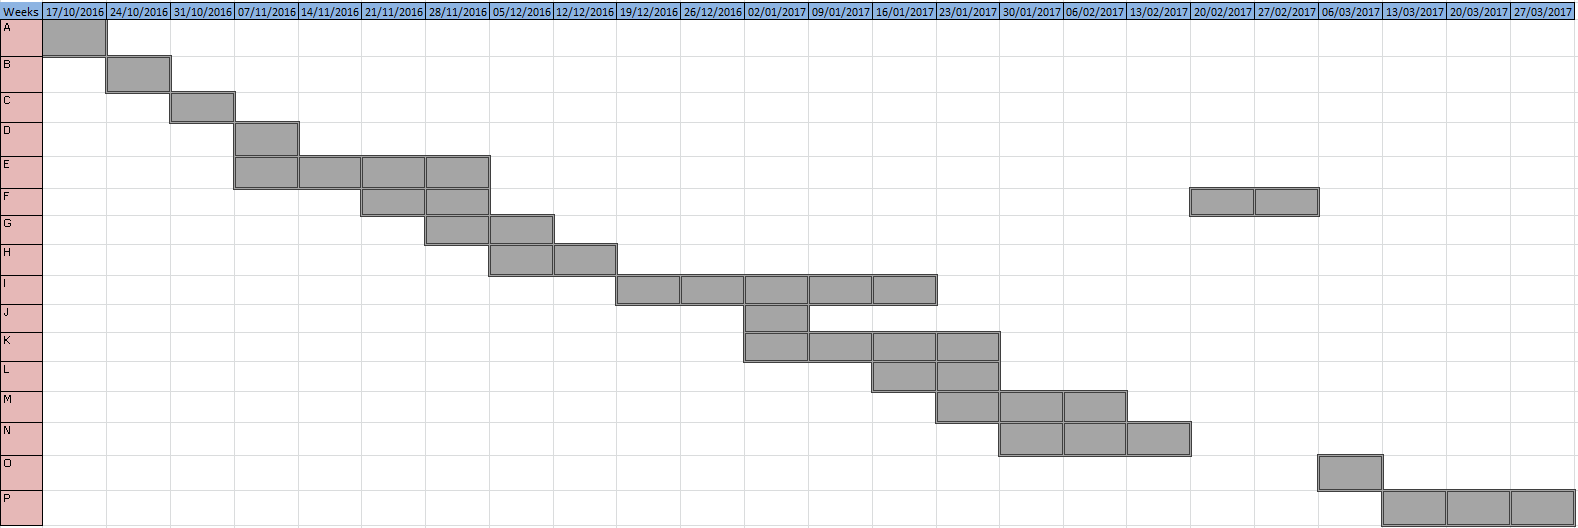
\includegraphics[width =700px, height=300px]{../Graphics/TimePlanUpdated2.png} \par
\hspace*{-1cm}

\end{landscape}

\newpage

\begin{changemargin}{\CMwidth}{\CMheight} 

\addcontentsline{toc}{section}{References}
\begin{thebibliography}{9}

\bibitem{cite0} Max D. Gunzburger, Janet S. Peterson \emph{Finite Element Methods} \url{https://people.sc.fsu.edu/~jburkardt/classes/fem\_2011/chapter1.pdf}

\bibitem{HandPRefinements} Adaptive Finite Element Techniques \url{http://www.cs.rpi.edu/~flaherje/pdf/fea8.pdf}

\bibitem{RRefinement} Scott McRae \emph{r-Refinement grid adaptation algorithms and issues}

\bibitem{DolsakPaper91} Bojan Dolsak and Anton Jezernik \emph{Mesh generation expert system for engineering analysis with FEM}

\bibitem{DolsakPaper94} Bojan Dolsak, Anton Jezernik \emph{A knowledge base for finite element mesh design} Artificial Intelligence in Engineering 9 (1994)

\bibitem{appOfILPToFEMeshDesign} Bojan Dolsak, Stephen Muggleton \emph{The Application of Inductive Logic Programming to Finite Element Mesh Design}

\bibitem{ConsultRuleIntelltSystemFE} Bojan Dolsak, Frank Reig, Reinhard Hackenschmidt \emph{Consultative Rule-Based Intelligent System for Finite Element Type Selection} Research Gate 2016

\bibitem{TraditionalHybridRefinement} Paul Dvorak \emph{Two meshing methods are better than one} \url{http://machinedesign.com/archive/two-meshing-methods-are-better-one}

\bibitem{NeuralNetworks} Larry Manevitz, Malik Yousef, Dan Givoli \emph{Automatic Mesh Generation (for Finite Element Method) Using Self-Organising Neural Networks}

\bibitem{caseBasedReasoning}Abid Ali Khan, Imran Ali Chaudhry2 \& Ali SaroshCase \emph{Case Based Reasoning Support for Adaptive Finite Element Analysis: Mesh Selection for an Integrated System}

\bibitem{MuggletonILP} Stephen Muggleton \emph{Inductive Logic Programming}

\bibitem{Golem} \url{http://www-ai.ijs.si/~ilpnet2/systems/golem.html}

\bibitem{ILPYoutubeLecture}Stephen Muggleton \emph{Logic based and Probabilistic Symbolic Learning} \url{https://www.youtube.com/watch?v=4CwdO5dWW98}

\bibitem{DittmerMeshQualityMet} Jeremy P. Dittmer, C. Greg Jensen, Michael Gottschalk, and Thomas Almy \emph{Mesh Optimisation Using a Genetic Algorithm to Control Mesh Creation Parameters}

\bibitem{PoorFEElementShapes} \url{http://danielpeter.github.io/rays.html}

\bibitem{cite03} Lina Vasiliauskiene, Romualdas BAUŠYS \emph{Intelligent Initial Finite Element Mesh Generation for Solutions of 2D Problems} INFORMATICA, 2002, Vol. 13, No. 2, 239–250 2002

\bibitem{cite04} E.Bellengera,Y.Benhafidb, N.Troussierb \emph{Framework for controlled cost and quality of assumptions in finite element analysis} Finite Elements in Analysis and Design 45 (2009) 25--36

\bibitem{IntroductionToFE} G. P. Nikishkov \emph{INTRODUCTION TO THE FINITE ELEMENT METHOD} \url{http://homepages.cae.wisc.edu/~suresh/ME964Website/M964Notes/Notes/introfem.pdf}

\bibitem{LISAManual} \url{http://www.lisafea.com/pdf/manual.pdf}

\bibitem{cite06}Nam-Ho Kim \emph{STRUCTURAL DESIGN USING FINITE ELEMENTS} http://web.mae.ufl.edu/nkim/eas6939/Opt\_FEM.pdf

\bibitem{cite07}\emph{Type of Finite Elements and Steps in FEA Process}\\
http://highered.mheducation.com/sites/dl/free/0073398144/934758/\\Ch07TypesOfFiniteElementsAndStepsInFEAProcess.pdf 

\bibitem{cantileverBeam} \url{https://www.quora.com/What-is-the-cantilever-beam-What-is-the-advantages-and-disadvantages-of-it}

\bibitem{LISAWebsite} \url{http://www.lisafea.com/purchase.html}

\bibitem{Doxygen} \url{http://www.stack.nl/~dimitri/doxygen/} 

\bibitem{ElementShapeQuality} \url{https://caeai.com/blog/will-poorly-shaped-elements-really-affect-my-solution}

\bibitem{AnsysCost} \url{http://mscnastrannovice.blogspot.co.uk/2013/04/how-much-does-ansys-cost.html}

\bibitem{HighStressCorner} \url{http://www.engineeringanalysisservices.com/moving-mesh-fea-analysis.php}

\bibitem{CSharpConvexHull} \url{http://loyc.net/2014/2d-convex-hull-in-cs.html}

\bibitem{YoungsModulus} \url{http://physicsnet.co.uk/a-level-physics-as-a2/materials/young-modulus/}

\bibitem{PossionsRatio} \url{http://silver.neep.wisc.edu/~lakes/PoissonIntro.html}

\bibitem{DelaunyTriangles} Jonathan Richard Shewchuk \emph{Delaunay Refinement Algorithms
for Triangular Mesh Generation} \url{https://people.eecs.berkeley.edu/~jrs/papers/2dj.pdf}

\bibitem{RotatingDiskFE} Eliannah Hunderfund and Professor Ernesto Gutierrez-Miravete Rensselaer 
\emph{Finite Element Analysis of a Rotating Disk}


\bibitem{PaperMillSpeeds} \url{http://www.pulpandpapercanada.com/news/coupling-changes-cut-paper-machinery-maintenance-1000108660}

\bibitem{Centripetal} \url{http://www.engineeringtoolbox.com/centripetal-acceleration-d_1285.html}

\bibitem{VisualStudioMaintainIndex} \url{https://msdn.microsoft.com/en-gb/library/bb385914.aspx}


\end{thebibliography}
\appendix

\section{Element Types within LISA}
Here are shown the the visual specifications LISA provides for the ordering and layout of nodes for defining each type of element supported. Each of these types can be classified using the

\begin{figure}[!h]
\centering
\begin{subfigure}{.5\textwidth}
  \centering
  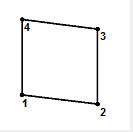
\includegraphics[width=0.3\linewidth]{../Graphics/LISA-quad4.png}
  \caption{quad4 element}
  \label{fig:sub1}
\end{subfigure}%
\begin{subfigure}{.5\textwidth}
  \centering
  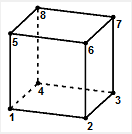
\includegraphics[width=0.3\linewidth]{../Graphics/LISA-hex8.png}
  \caption{hex8 element}
  \label{fig:sub2}
\end{subfigure}
\label{fig:test}
\end{figure}


\begin{figure}[!h]
\centering
\begin{subfigure}{.5\textwidth}
  \centering
  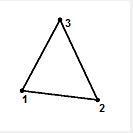
\includegraphics[width=0.3\linewidth]{../Graphics/LISA-tri3.png}
  \caption{Specification for node ordering of tri3 element within LISA}
  \label{fig:sub1}
\end{subfigure}%
\begin{subfigure}{.5\textwidth}
  \centering
  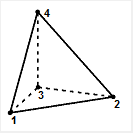
\includegraphics[width=0.3\linewidth]{../Graphics/LISA-tet4.png}
  \caption{tet4 element}
  \label{fig:sub2}
\end{subfigure}
\label{fig:test}
\end{figure}


\begin{figure}[!h]
\centering
\begin{subfigure}{.5\textwidth}
  \centering
  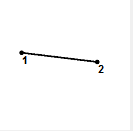
\includegraphics[width=0.3\linewidth]{../Graphics/LISA-line2.png}
  \caption{line2 element}
  \label{fig:sub1}
\end{subfigure}%
\begin{subfigure}{.5\textwidth}
  \centering
  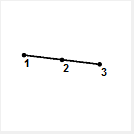
\includegraphics[width=0.3\linewidth]{../Graphics/LISA-line3.png}
  \caption{line3 element}
  \label{fig:sub2}
\end{subfigure}
\label{fig:test}
\end{figure}

\section{Calculating Centripetal Force For Paper Mill}
Assuming a constant speed of the paper mill disk at  the following standard calculation was done to compute a forces that could be specified for different elements in order to simulate the effects on the model.

F = m $\omega^2$ r\\ 

where: \\ 
m - mass of object \\ 
r - radius from centre \\ 
$\omega$ - angular velocity (radians per second)

Using the following values for each variable for the plates forming the outside of the paper mill disk the force could be calculated as:

mass- paper mill is made of steel with each plate having a volume of approximately $24cm^3$ which gives a mass of
188 grams




\cite{Centripetal}

\section{Input and output files}
Below can be seen the format of the input files for the system (A LISA .liml and a .json edge definition file\\

\begin{figure}[!h]
\centering
\begin{subfigure}{.5\textwidth}
  \centering
  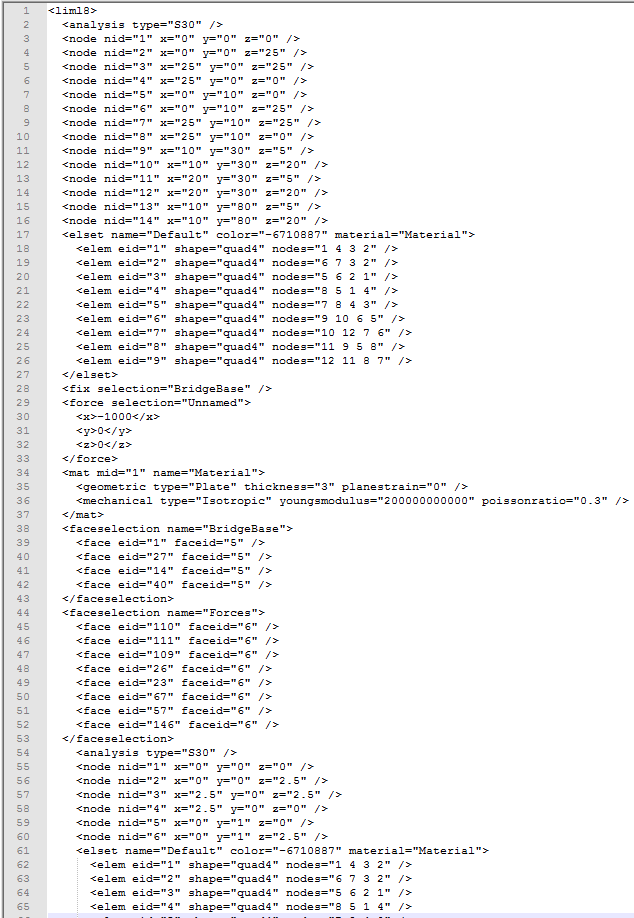
\includegraphics[width=0.6\linewidth]{../Graphics/limlFileLayout.png}
  \caption{Cut down .liml file to show general content which largely defined the schema for the systems data model}
  \label{fig:sub1}
\end{subfigure}%
\begin{subfigure}{.5\textwidth}
  \centering
  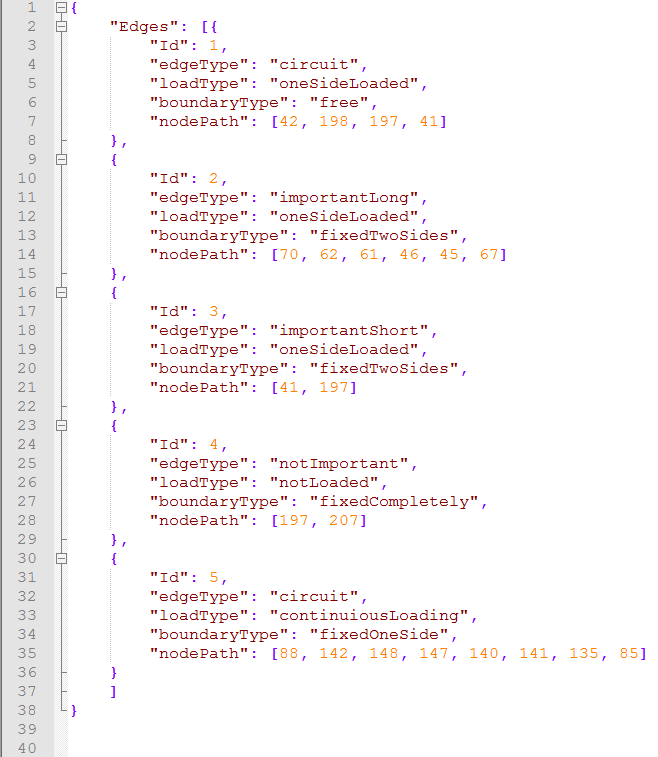
\includegraphics[width=0.8\linewidth]{../Graphics/jsonEdgeFileLayout.png}
  \caption{A json file containing the edges of interest specified by an engineer, this is parsed and the rules are applied to determine the models meshing based on the input}
  \label{fig:sub2}
\end{subfigure}
\label{fig:test}
\end{figure}


\section{Software Quality Metrics}


\begin{figure}
  \centerline{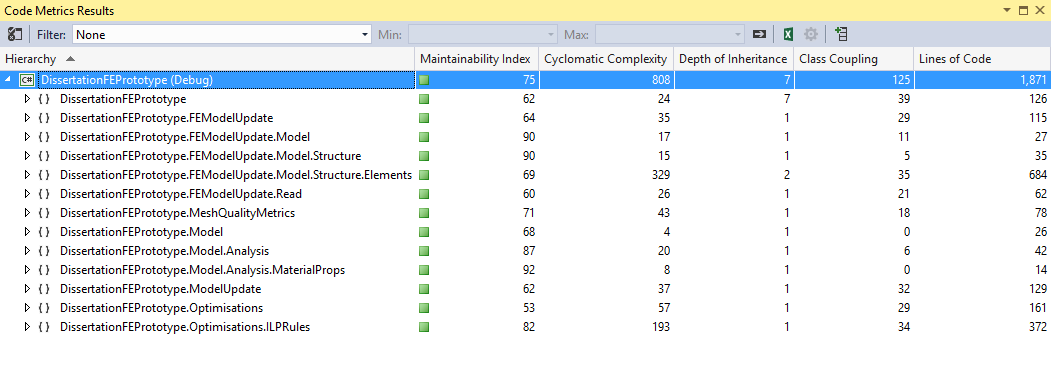
\includegraphics[width=165mm, scale=0.5]{../Graphics/softwareQualityMetrics.png}}
  \caption{The metrics calculated by visual studio for all high level modules in the system}
  \label{fig:boat1}
\end{figure}

\begin{figure}
  \centerline{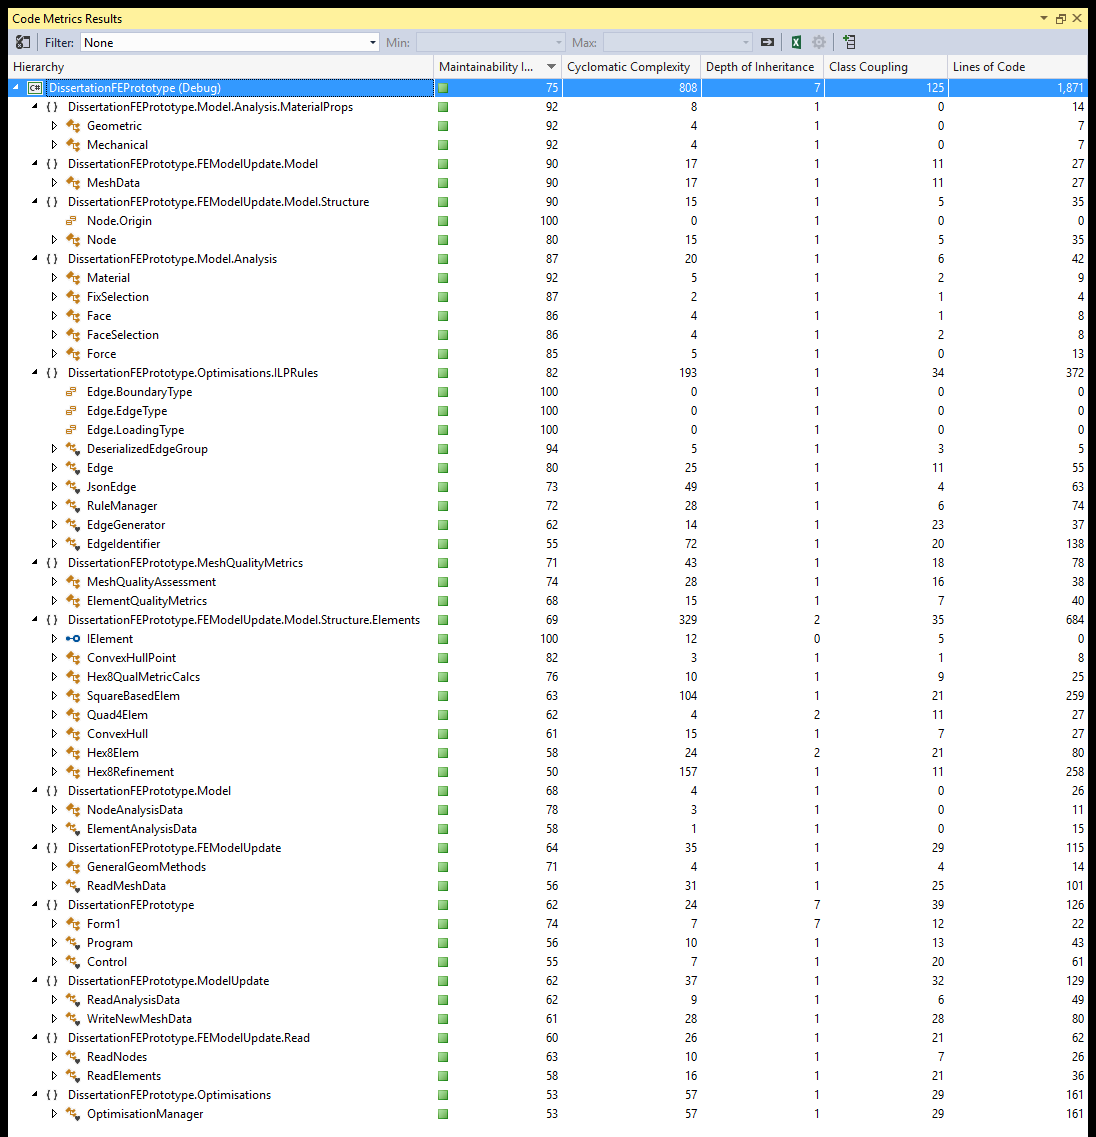
\includegraphics[width=165mm, scale=0.5]{../Graphics/qualityMetricsExpanded.png}}
  \caption{The metrics calculated by visual studio for the all classes in the final system}
  \label{fig:boat1}
\end{figure}



\end{changemargin}
